\section{OSR in LLVM}
\label{se:osr-llvm}

In this section we discuss our implementation of the approach described in \ref{se:overview} in \tinyvm, a proof-of-concept virtual machine we developed as a playground to exercise our OSR techniques. TinyVM is based on LLVM's MCJIT compiler and supports interactive invocation of LLVM IR functions either generated at run-time or loaded from disk. The main design goal behind TinyVM is the creation of an interactive environment for IR manipulation and JIT-compilation of functions: for instance, it allows the user to insert OSR points in loaded functions, run optimization passes on them or display their CFGs, repeatedly invoke a function for a specified amount of times and so on. TinyVM supports dynamic library loading and linking, and comes with a helper component for MCJIT that simplifies tasks such as handling multiple IR modules, symbol resolution in presence of multiple versions of a function, and tracking native code and other machine-level generated object such as Stackmaps.

To explain how \tinyvm\ works, we consider the toy example of \myfigure\ref{fi:isord-example}. Function {\tt isord} checks whether an array of numbers is sorted according to some ordering given by a comparator. We explore how to dynamically divert control to a faster version where the comparator is inlined if the number of iterations exceeds a certain threshold. To achieve this goal, we use deferred compilation by instrumenting {\tt isord} in \tinyvm\ with an open OSR, as shown in \myfigure\ref{fig:isordfrom}.

\ifdefined\noauthorea
\begin{figure}[t]
\begin{center}
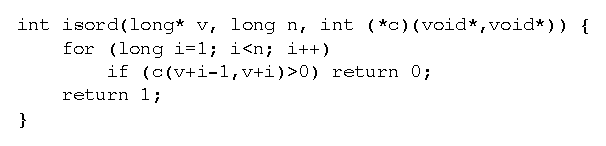
\includegraphics[width=0.9\columnwidth]{figures/isord-example/isord.eps}
\caption{\protect\label{fig:isordfrom} OSR instrumentation of base function in LLVM IR (in grey). The OSR is fired at the beginning of the loop body after 1000 iterations.
}
\end{center}
\end{figure}
\fi

\ifdefined\noauthorea
\begin{figure}[t]
\begin{center}
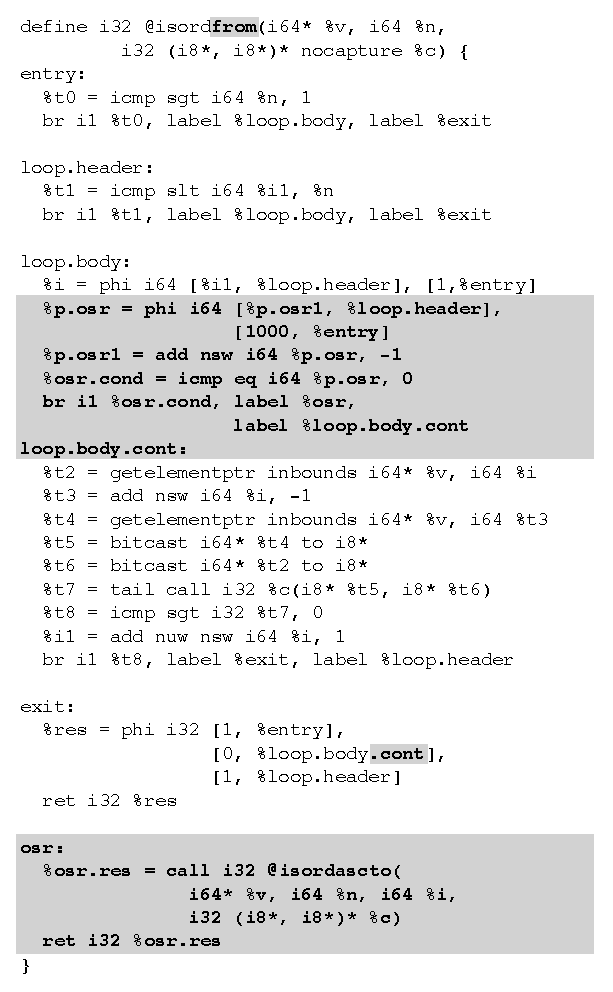
\includegraphics[width=0.9\columnwidth]{figures/isordfrom/isordfrom.eps}
\caption{\protect\label{fig:isordfrom} IR version of base function {\tt isord} (\myfigure\ref{fi:isord-example}) instrumented for resolved OSR. The OSR is fired at the beginning of the loop body after 1000 iterations. Additions resulting from the instrumentation are in grey.
}
\end{center}
\end{figure}
\fi

\ifdefined\noauthorea
\begin{figure}[t]
\begin{center}
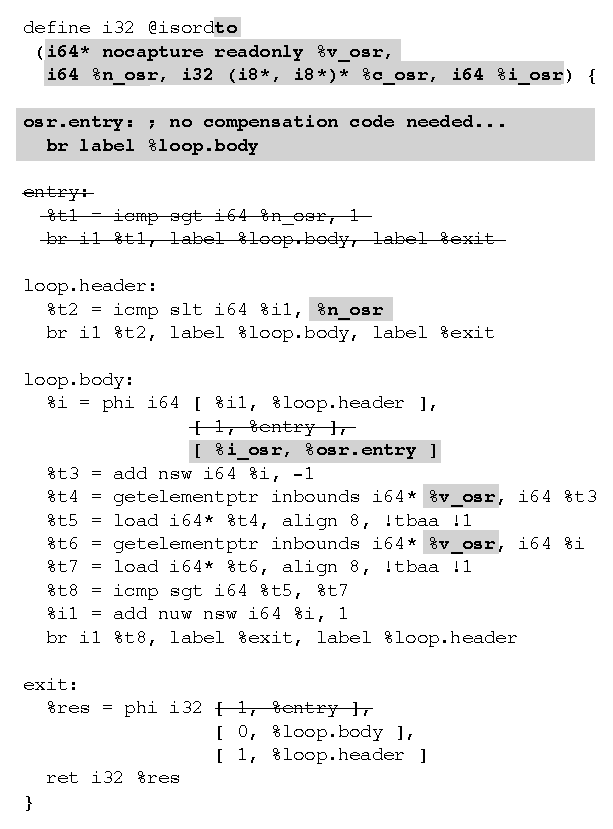
\includegraphics[width=0.9\columnwidth]{figures/isordascto/isordascto.eps}
\caption{\protect\label{fig:isordascto} OSR instrumentation (in grey) of faster variant {\tt isordasc} (\myfigure\ref{fi:osr-dynamics}) in LLVM IR. The original function entry block is unreachable after instrumentation and eliminated (struck-through code fragments).
}
\end{center}
\end{figure}
\fi

\ifdefined\noauthorea
\begin{figure}[t]
\begin{center}
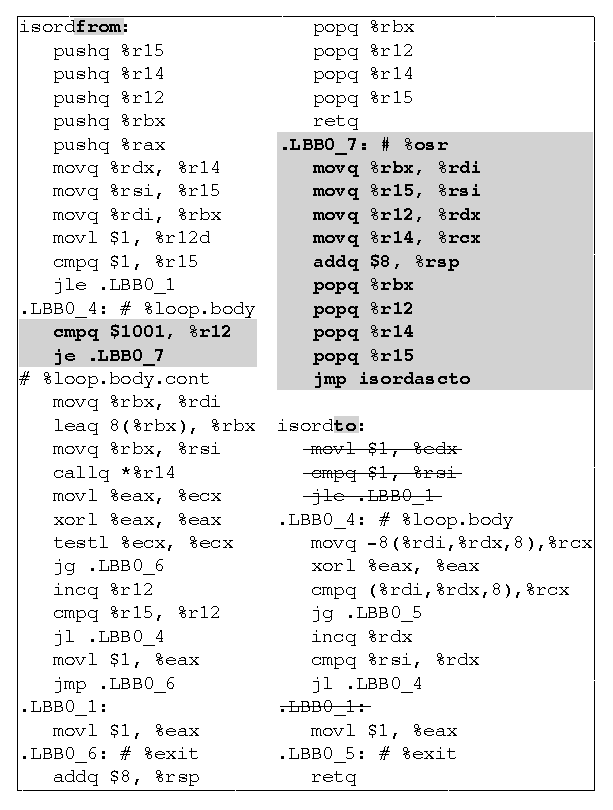
\includegraphics[width=0.9\columnwidth]{figures/isordx86-64/isordx86-64.eps}
\caption{\protect\label{fig:isordx86-64} OSR-instrumented functions {\tt isordfrom} (base) and {\tt isordascto} (faster continuation) after IR to x86-64 lowering in LLVM. For the sake of comparison with the native code that would be generated for the original non-OSR versions, additions resulting from the IR instrumentation are in grey, while removals are struck-through.}
\end{center}
\end{figure}
\fi

%\subsection{Resolved OSR Points}

%\subsection{Open OSR Points}
  

  
  
  
  